\documentclass[tikz,border=6pt]{standalone}
\usepackage{amsmath,amssymb,amsfonts,xcolor}
\newcommand{\D}{\mathbb{D}}
\begin{document}
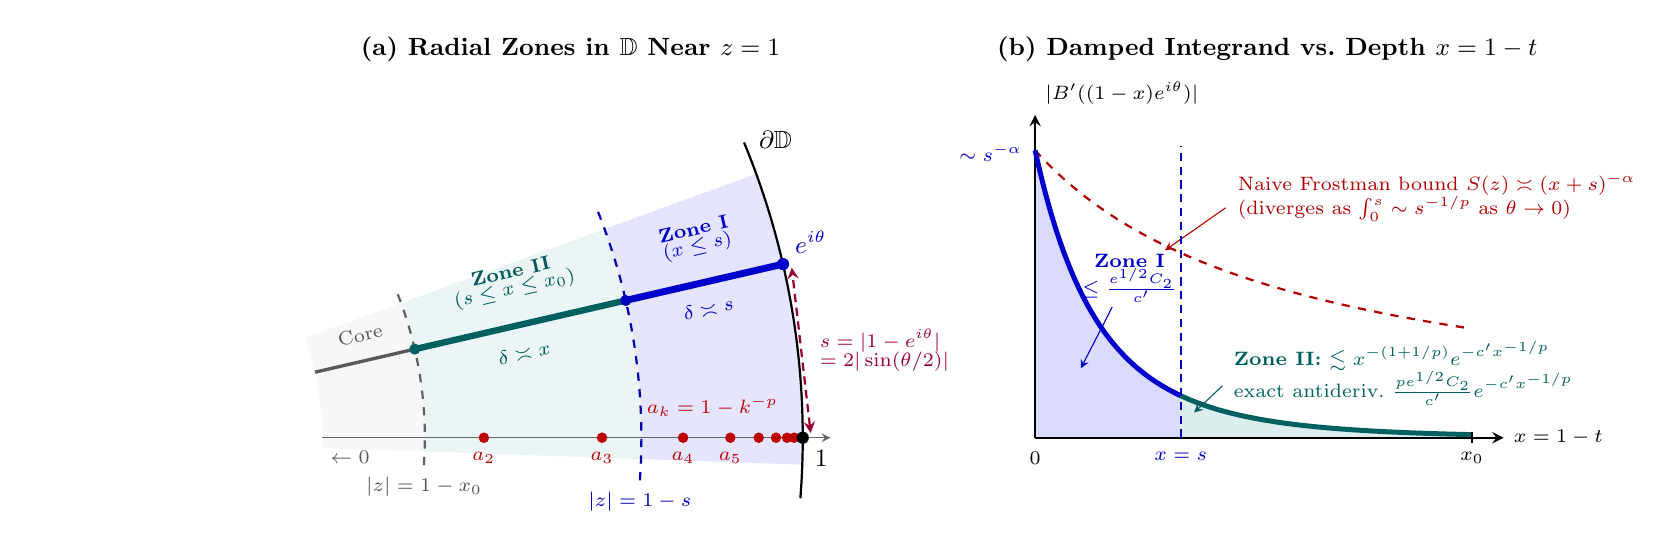
\begin{tikzpicture}[>=stealth, font=\small]
  % =========================================================================
  % PANEL (a): Magnified Geometry in D near z = 1 (center of circle at (-3.6, 1.0), R = 9.8)
  % =========================================================================
  \begin{scope}
    % Title for Panel (a)
    \node[font=\bfseries\small, anchor=south] at (3.25, 5.65) {(a) Radial Zones in $\D$ Near $z = 1$};

    % Subtle shaded core sector inside unit disk (between r = 3.7 and r = 5.0)
    \fill[gray!6] (-3.6, 1.0) ++(-2:3.7) arc (-2:20:3.7)
      -- ++(20:1.3) arc (20:-2:5.0) -- cycle;

    % Zone II radial band shading (between r = 5.0 and r = 7.75)
    \fill[teal!8] (-3.6, 1.0) ++(-2:5.0) arc (-2:20:5.0)
      -- ++(20:2.75) arc (20:-2:7.75) -- cycle;

    % Zone I radial band shading (between r = 7.75 and r = 9.8)
    \fill[blue!10] (-3.6, 1.0) ++(-2:7.75) arc (-2:20:7.75)
      -- ++(20:2.05) arc (20:-2:9.8) -- cycle;

    % Dashed arc |z| = 1 - x_0 (r = 5.0 from (-3.6, 1.0))
    \draw[dashed, gray!75!black, thick] (-3.6, 1.0) ++(-4:5.0) arc (-4:22:5.0);
    \node[gray!65!black, font=\scriptsize, anchor=north] at (1.39, 0.62) {$|z| = 1 - x_0$};

    % Dashed crossover arc |z| = 1 - s (r = 7.75 from (-3.6, 1.0))
    \draw[dashed, blue!70!black, thick] (-3.6, 1.0) ++(-4:7.75) arc (-4:22:7.75);
    \node[blue!70!black, font=\scriptsize, anchor=north] at (4.13, 0.44) {$|z| = 1 - s$};

    % Unit circle arc \partial\D (r = 9.8 from (-3.6, 1.0))
    \draw[thick, black] (-3.6, 1.0) ++(-4.5:9.8) arc (-4.5:22.5:9.8);
    \node[black, font=\small, anchor=west] at (5.52, 4.78) {$\partial\D$};

    % Positive real axis (\theta = 0): y = 1.0 from x = 0.1 to x = 6.55
    \draw[->, gray!80!black] (0.1, 1.0) -- (6.55, 1.0);
    \node[font=\scriptsize, gray!70!black, anchor=north] at (0.45, 0.95) {$\leftarrow 0$};

    % Polynomially clustering Blaschke zeros a_k = 1 - k^{-p} on [0, 1)
    \foreach \xpos/\lbl in {2.15/$a_2$, 3.65/$a_3$, 4.68/$a_4$, 5.28/$a_5$, 5.64/{}, 5.86/{}, 6.00/{}, 6.09/{}} {
      \fill[red!75!black] (\xpos, 1.0) circle (1.9pt);
      \ifx\lbl\empty\else
        \node[red!75!black, font=\scriptsize, anchor=north] at (\xpos, 0.94) {\lbl};
      \fi
    }
    \node[red!75!black, font=\scriptsize, anchor=south] at (5.05, 1.14) {$a_k = 1 - k^{-p}$};

    % Boundary point z = 1 at (6.2, 1.0)
    \fill[black] (6.2, 1.0) circle (2.2pt);
    \node[black, font=\small, anchor=north west] at (6.23, 0.96) {$1$};

    % Off-axis ray at angle \theta = 13 deg from (-3.6, 1.0):
    % Core segment: r from 3.7 to 5.0
    \draw[very thick, gray!70!black] (-3.6, 1.0) ++(13:3.7) -- ++(13:1.3);
    % Zone II segment: r from 5.0 to 7.75 (teal)
    \draw[line width=2.3pt, teal!75!black] (-3.6, 1.0) ++(13:5.0) -- ++(13:2.75);
    % Zone I segment: r from 7.75 to 9.8 (royal blue)
    \draw[line width=2.5pt, blue!80!black] (-3.6, 1.0) ++(13:7.75) -- ++(13:2.05);

    % Endpoint e^{i\theta} at (-3.6 + 9.8*cos(13), 1.0 + 9.8*sin(13)) = (5.949, 3.205)
    \fill[blue!80!black] (5.949, 3.205) circle (2.2pt);
    \node[blue!80!black, font=\small, anchor=south west] at (5.98, 3.22) {$e^{i\theta}$};

    % Crossover point (1 - s)e^{i\theta} at (3.951, 2.743)
    \fill[blue!75!black] (3.951, 2.743) circle (2.0pt);

    % Core boundary point (1 - x_0)e^{i\theta} at (1.272, 2.125)
    \fill[teal!75!black] (1.272, 2.125) circle (2.0pt);

    % Chord s = |1 - e^{i\theta}| = 2|\sin(\theta/2)|
    \draw[<->, densely dashed, purple!80!black, thick] (6.30, 1.06) -- (6.06, 3.16)
      node[midway, right=3pt, font=\scriptsize, purple!80!black, align=left] {$s = |1 - e^{i\theta}|$\\[-1pt]$= 2|\sin(\theta/2)|$};

    % Zone labels along the ray
    \node[teal!70!black, font=\scriptsize, rotate=13, align=center] at (2.52, 2.98) {\textbf{Zone II}\\[-2pt]$(s \le x \le x_0)$};
    \node[teal!70!black, font=\scriptsize, rotate=13] at (2.66, 2.08) {$\delta \asymp x$};

    \node[blue!80!black, font=\scriptsize, rotate=13, align=center] at (4.84, 3.52) {\textbf{Zone I}\\[-2pt]$(x \le s)$};
    \node[blue!80!black, font=\scriptsize, rotate=13] at (5.00, 2.64) {$\delta \asymp s$};

    \node[gray!65!black, font=\scriptsize, rotate=13] at (0.58, 2.30) {Core};
  \end{scope}

  % =========================================================================
  % PANEL (b): Radial Integrand Profile vs. Depth x = 1 - t
  % =========================================================================
  \begin{scope}[xshift=8.75cm]
    \node[font=\bfseries\small, anchor=south] at (3.35, 5.65) {(b) Damped Integrand vs.\ Depth $x = 1 - t$};

    % Shaded area under Pole-Free Bound in Zone I: X in [0, 1.85]
    \fill[blue!14] (0.4, 1.0)
      -- plot[domain=0:1.85, samples=45] ({0.4 + \x}, {1.0 + 3.65 * ((1 + 0.32*\x)^(-0.95)) * exp(-0.95*\x * ((1 + 0.25*\x)^(-0.45)))})
      -- (2.25, 1.0) -- cycle;

    % Shaded area under Pole-Free Bound in Zone II: X in [1.85, 5.55]
    \fill[teal!14] (2.25, 1.0)
      -- plot[domain=1.85:5.55, samples=65] ({0.4 + \x}, {1.0 + 3.65 * ((1 + 0.32*\x)^(-0.95)) * exp(-0.95*\x * ((1 + 0.25*\x)^(-0.45)))})
      -- (5.95, 1.0) -- cycle;

    % Axes
    \draw[->, thick] (0.4, 1.0) -- (6.35, 1.0) node[right, font=\scriptsize] {$x = 1 - t$};
    \draw[->, thick] (0.4, 1.0) -- (0.4, 5.10) node[above right, font=\scriptsize] {$|B'((1-x)e^{i\theta})|$};

    % Naive Frostman curve S(z) ~ (x + s)^{-\alpha} without exponential damping
    \draw[dashed, red!70!black, thick]
      plot[domain=0:5.55, samples=70] ({0.4 + \x}, {1.0 + 3.65 * ((1 + 0.32*\x)^(-0.95))});
    \node[red!70!black, font=\scriptsize, anchor=west, align=left] at (2.85, 4.05)
      {Naive Frostman bound $S(z) \asymp (x+s)^{-\alpha}$\\[-1pt](diverges as $\int_0^s \sim s^{-1/p}$ as $\theta \to 0$)};
    \draw[->, red!70!black, thin] (2.82, 3.92) -- (2.05, 3.38);

    % Pole-free damped bound e^{1/2} C_2 (x+s)^{-\alpha} \exp(-c x (x+s)^{-\alpha})
    \draw[line width=1.8pt, blue!80!black]
      plot[domain=0:1.85, samples=45] ({0.4 + \x}, {1.0 + 3.65 * ((1 + 0.32*\x)^(-0.95)) * exp(-0.95*\x * ((1 + 0.25*\x)^(-0.45)))});
    \draw[line width=1.8pt, teal!75!black]
      plot[domain=1.85:5.55, samples=65] ({0.4 + \x}, {1.0 + 3.65 * ((1 + 0.32*\x)^(-0.95)) * exp(-0.95*\x * ((1 + 0.25*\x)^(-0.45)))});

    % Crossover vertical line at x = s (X = 0.4 + 1.85 = 2.25)
    \draw[densely dashed, blue!75!black, thick] (2.25, 1.0) -- (2.25, 4.70);
    \node[below, font=\scriptsize, blue!80!black] at (2.25, 0.94) {$x = s$};
    \node[below, font=\scriptsize] at (0.4, 0.94) {$0$};
    \node[below, font=\scriptsize] at (5.95, 0.94) {$x_0$};
    \draw[thick] (5.95, 0.93) -- (5.95, 1.07);

    % Peak label at x = 0
    \node[left, font=\scriptsize, blue!80!black] at (0.36, 4.62) {$\sim s^{-\alpha}$};

    % Annotations for Zone I and Zone II areas
    \node[blue!80!black, font=\scriptsize, align=center] at (1.60, 3.02) {\textbf{Zone I}\\[-1pt]$\le \frac{e^{1/2}C_2}{c'}$};
    \draw[->, blue!80!black, thin] (1.38, 2.66) -- (0.98, 1.88);
    \node[teal!75!black, font=\scriptsize, anchor=west, align=left] at (2.80, 1.82)
      {\textbf{Zone II:} $\lesssim x^{-(1+1/p)} e^{-c' x^{-1/p}}$\\[-1pt]exact antideriv.\ $\frac{p e^{1/2} C_2}{c'} e^{-c' x^{-1/p}}$};
    \draw[->, teal!75!black, thin] (2.78, 1.66) -- (2.42, 1.32);
  \end{scope}
\end{tikzpicture}
\end{document}
